\documentclass{beamer}
\usepackage[latvian]{babel}
\usepackage[pangram]{blindtext}
%\usetheme{Pittsburgh}
\usepackage[utf8]{inputenc}
\usepackage[T1]{fontenc}
\usepackage{graphicx}
\usepackage{tikz}
\usepackage{makecell}
\usepackage{amsmath}
\usepackage{amssymb}
\usepackage{siunitx}
\usepackage{multirow}
\usepackage{longtable}
\usepackage{subfig}
\usepackage{ragged2e}
%\usepackage{listings}
\usetikzlibrary{positioning, fit, shapes, calc, angles, intersections, quotes, babel, through}
\tikzset{point/.style={circle, inner sep=0pt, minimum size=3pt, fill=red}}
\newlength{\pvlength}

\title{Virsotnes kvarku pāra sabrukšanas ceļā radušos krāsu plūsmu pētījumi ar 13 TeV CERN LHP KMS eksperimentā}
\author{Viesturs Veckalns}
\institute{Rīgas Tehniskā universitāte}
\date{2018. g. 7. decembris}
\setbeamercolor{title}{fg=black}                            
\setbeamercolor{date}{fg=black}
\setbeamerfont{footline}{size=\fontsize{8}{5}\selectfont}
\setbeamerfont{date}{size=\fontsize{6}{4}\selectfont}
\setbeamerfont{title}{series=\bfseries}


\usepackage{xparse,calc}
%\logo{\raisebox{-6cm}{\includegraphics[width=1cm]{CMS_logo_May2014-eps-converted-to.pdf}}}

%\makeatletter
\input{presentation/presdefinitions.tex}
\usepackage{xspace}
\newcommand{\ttbar}{\ensuremath{t\overline{t}}\xspace}
\newcommand{\fbinv}{\ensuremath{\text{fb}^{-1}}\xspace}
\newcommand{\PW}{$W$\xspace}
\newcommand{\cPZ}{$Z$\xspace}

\begin{document}
{
  \usebackgroundtemplate{\includegraphics[width=\paperwidth]{presentation/pamats1.jpg}}%
  \setbeamertemplate{footline}{}
  \logo{}
  \begin{frame}
    \fitimage{%
      \titlepage
      %\blindenumerate[2]
    }{example-image-a}
  \end{frame}
}


\begin{frame}{Krāsu plūsma \ttbar sabrukuma procesā}
  \centering
  \includegraphics[width=0.85\textwidth]{presfig/ttbar_cf_labels_lv.pdf}
\end{frame}

\begin{frame}{Šķērsgriezumus}
  746 pb pie $\sqrt{s}=13$ TeV
  \centering
  \includegraphics[width=0.85\textwidth]{fig/tt_curve_toplhcwg_sep18.pdf}
\end{frame}

\begin{frame}{Pāra rašanās}
  \centering
  \def\twidth{0.4}
  \begin{minipage}{\twidth\paperwidth}
    \includegraphics[width=\textwidth]{fig/top_quark_pair_prod_gfusion}
    \label{fig:top_quark_production}
  \end{minipage}
  \begin{minipage}{\twidth\paperwidth}
    \includegraphics[width=\textwidth]{fig/top_quark_pair_prod_gluon}
    \label{fig:top_quark_production2}
  \end{minipage}

\end{frame}

\begin{frame}{Hadronizācija}
  \centering
  \includegraphics[width=0.8\textwidth]{fig/combinationlv.pdf}
\end{frame}

\begin{frame}{Hadronizācija}
  \centering
  \includegraphics[width=0.8\textwidth]{fig/colour_field_fulllv.pdf}
\end{frame}

\begin{frame}{Komandas biedri}
  \begin{itemize}
  \item Martijn Mulders (CERN)
  \item Pedro Silva (CERN)
  \item Markus Seidel (CERN)
  \end{itemize}
\end{frame}

\begin{frame}{Saturs}
  \begin{enumerate}
  \item Eksperimentālais aprīkojums
  \item Vilkmes leņķa metodoloģija
  \item Atlocīšana
  \item ``LEP'' metodoloģija
  \item Hipotēžu pārbaude
  \end{enumerate}
\end{frame}

\begin{frame}{Novitāte}
  \begin{description}
  \item[vilkmes leņķis]
    Tevatrona D\O\ eksperiments \scriptsize(Phys.Rev. D83 (2011) 092002)\normalsize, ATLAS Run I \scriptsize(Phys.Lett. B750 (2015) 475-493)\normalsize\ un Run II \scriptsize(Eur.Phys.J. C78 (2018) no.10, 847)\normalsize\\
    Pirmo reizi tiek izmantos KMS. KMS 4T solenoīds pret ATLAS 2T solenoīdu.
  \item[``LEP'' metodoloģija]
    LEP eksperiments OPAL \scriptsize(Eur.Phys.J. C45 (2006) 291-305)\normalsize, DELPHI \scriptsize(Eur.Phys.J. C51 (2007) 249-269)\normalsize, L3 \scriptsize(Phys.Lett. B561 (2003) 202-212)\normalsize\\
    Nekad nav izmantota LHP
  \item[pirmais pienesums no Latvijas]
  \end{description}
  
\end{frame}


\begin{frame}{Lielais hadronu paātrinātājs}
  \centering
  \includegraphics[width=0.5\textwidth]{fig/LHC_underground.png}%
  \includegraphics[width=0.5\textwidth]{fig/CERNacceleratorcomplex.jpg}\\
  sinhrotrons - nemainīgs radiuss, bet mainīga frekvence (pretēji ciklotronam)\\
  uzkrāšanas riņķis (storage ring)\\
  supravadoši magnēti (8T, <2K)
\end{frame}


\begin{frame}{Kompaktais mionu solenoīds}
  \centering
  \includegraphics[width=1\textwidth]{fig/cms_160312_06lv.pdf}
  (J. Phys.: Conf. Ser. 513 022032)
\end{frame}

\begin{frame}{Lietotās mērvienības}
  \centering
  \begin{minipage}{0.55\textwidth}
    \includegraphics[width=1\textwidth]{fig/coordinates/coordinateslv.pdf}
  \end{minipage}%
  \hspace{0.5cm}%
  \begin{minipage}{0.35\textwidth}
    pseidostraujums $\eta$
    \begin{equation*}
      \eta\equiv-\ln\left(\frac{\theta}{2}\right)
    \end{equation*}
    straujums $y$
    \begin{equation*}
      y\equiv\ln\left(\frac{E+p_{L}}{E-p_{L}}\right)
    \end{equation*}
  \end{minipage}
\end{frame}

\begin{frame}{Notikumu atlase}
  \def\twidth{0.3}
  \begin{minipage}{\twidth\paperwidth}
    \includegraphics[width=\textwidth]{fig/ttbar_cf.pdf}
    \label{fig:top_quark_production}
  \end{minipage}%
  \begin{minipage}{0.6\paperwidth}
    \begin{itemize}
    \item 1 leptons ($e^{\pm}$/$\mu^{\pm}$), \scriptsize$p_{T}> \SI{34}{GeV}/\SI{26}{GeV}$, $\left|\eta\right| < \SI{2.1}{}/\SI{2.6}{}$, HLT\_Ele32\_eta2p1\_WPTight\_Gsf\_v/ HLT\_IsoMu24\_v vai HLT\_IsoTkMu24\_v \normalsize
    \item 4 strūklas \scriptsize $p_{T}>\SI{30}{GeV}$, $\left|\eta\right|<2.4$, nav pārklājuma ar leptonu ($\Delta R>0.4$)\normalsize
      \begin{itemize}
      \item[-] 2 vieglās strūklas
      \item[-] 2 $b$-atzīmētās strūklas
      \end{itemize}
      \vspace{0.5cm}
      \centering
      \includegraphics[width=0.6\textwidth]{fig/CMS-BTV-16-002_Figure_001.pdf}
    \end{itemize}
  \end{minipage}
\end{frame}

\begin{frame}{Notikumu atlase}
  \centering
  \includegraphics[width=0.8\textwidth]{fig/histos/L/reco/L_reco_selection.png}
\end{frame}

\section{Vilkmes leņķis}

\begin{frame}[fragile]{Vilkmes leņkis}
  \begin{overprint}
    \onslide<1>
    
    \onslide<2>
    1. strūklas vilkme uz 2. strūklu
    
    \onslide<3>
    Vilkmei ir gadījuma orientācija, ja strūklas nav saistītas
  \end{overprint}
  %  \includegraphics[width=0.7\paperwidth]{example-image-a};

  
  \begin{overlayarea}{\linewidth}{0.7\paperheight}
    \centering
    \begin{tikzpicture}
      \pgfmathsetmacro{\length}{sqrt(0.8^2 + 0.9^2)}
      \setlength{\pvlength}{\length cm}
      \input{presfig/pull_angle_templ.tex}
      \node(space) at (0.0, 4.5){};
      \only<1>{
        \def\angle{45}
        \coordinate (add) at ({(cos(\angle)*\pvlength}, {sin(\angle)*\pvlength});
        \coordinate (vp) at ($(jet1) + (add)$);
        \node[rectangle callout, fill=gray!20,
          callout absolute pointer={($(jet1) + (0.1, 0.1)$)}, align = center] at (-2.5, 3.0) {vilkmes leņķis}; 
        \node[rectangle callout, fill=gray!20,
          callout absolute pointer={($(vp) + (0.0, 0.45)$)}, align = center] at (-1.5, 4.0) {vilkmes vektors};
        \draw[->](jet1)--(vp) node[at end, above]{$\vec{v}_{p}$}; 
        \draw   pic [draw, angle radius=2.5mm, angle eccentricity = 1.8, "$\theta_{p}$" font = \tiny] {angle=jet2--jet1--vp};
        \node(a4)[text width = 3cm, scale=0.9] at (-0.2, -0.6)[anchor = east]{
          \begin{equation*}
            \vec{v}_{p}=\sum_{i\in J}\frac{p^{T}_{i}|\vec{r}_{i}|}{p^{T}_{J}}\vec{r}_{i}
          \end{equation*}
        };
      }
      \only<2>{
        \draw[fill=black] (jet1) + (0.2, -0.5) circle (1pt); 
        \draw[fill=black] (jet1) + (0.2, 0.5) circle (1pt); 
        \draw[fill=black] (jet1) + (0.3, -0.1) circle (1pt); 
        \draw[fill=black] (jet1) + (0.4, 0.1) circle (2pt); 
        \draw[fill=black] (jet1) + (0.4, -0.1) circle (1pt); 
        \draw[fill=black] (jet1) + (0.6, -0.0) circle (1pt); 
        \draw[fill=black] (jet1) + (0.7, 0.1) circle (1pt); 

        \def\angle{30}
        \coordinate (add) at ({(cos(\angle)*\pvlength}, {sin(\angle)*\pvlength});
        \coordinate (vp) at ($(jet1) + (add)$);
        \draw[->, color = red](jet1)--(vp) node[at end, above]{$\vec{v}_{p}$}; 
        \draw   pic [draw, angle radius=2.5mm, angle eccentricity = 1.8] {angle=jet2--jet1--vp};
      }
      \only<3>{
        \def\angle{100}
        \coordinate (add) at ({(cos(\angle)*\pvlength}, {sin(\angle)*\pvlength});
        \coordinate (vp) at ($(jet1) + (add)$);
        \draw[->, color = blue](jet1)--(vp) node[at end, above]{$\vec{v}_{p}$}; 
        \draw   pic [draw, angle radius=2.5mm] {angle=jet2--jet1--vp};
      }

    \end{tikzpicture}
  \end{overlayarea}
  \centering
  \tiny Gallichio et al ``Seeing in Color: Jet Superstructure'' (Phys.Rev.Lett. 105 (2010) 022001)
\end{frame}

\begin{frame}{Notikuma attēls}\centering
  \includegraphics[width=0.8\textwidth]{fig/individual_plots/reco_allconst_total_1111_DeltaR_2p846131_pull_angle_1p964620.png}
  \\vilkmes leņķis 1,96 rad.
\end{frame}

\begin{frame}{Daļiņas KMS detektorā}
  \centering
  \includegraphics[width=0.8\textwidth]{fig/cmspf.png}\\
  Daļiņu plūsmas rekonstrukcija, JINST 12 (2017) no.10, P10003
\end{frame}

\begin{frame}{Krāsu okteta $W$ bozona modelis}
  \centering
  \includegraphics[width=0.5\textwidth]{fig/ttbar_cf_flip.pdf}\\
  \vspace{0.5cm}
  \includegraphics[width=0.5\textwidth]{presfig/cflip_creation.pdf}
\end{frame}

\begin{frame}{Vilkmes vektora dimensijas}
  \centering
  \def\twidth{0.33}
  \setcounter{subfigure}{0}
  \begin{figure}
    \subfloat[$\eta$]{
      \includegraphics[width = \twidth\textwidth]{fig/histos/L/reco/PV/charge/allconst/L_eta_PV_allconst_reco_leading_jet.png}
    }%
    \subfloat[$\phi$]{
      \includegraphics[width = \twidth\textwidth]{fig/histos/L/reco/PV/charge/allconst/L_phi_PV_allconst_reco_leading_jet.png}
    }%
    \subfloat[modulis $\sqrt{\eta^{2} + \phi^{2}}$]{
      \includegraphics[width = \twidth\textwidth]{fig/histos/L/reco/PV/charge/allconst/L_mag_PV_allconst_reco_leading_jet.png}
    }
  \end{figure}
\end{frame}


\begin{frame}{Vilkmes leņķa distribūcijas}
  \centering
  \def\twidth{0.29}
  \setcounter{subfigure}{0}
  \begin{figure}
    \subfloat[vadošā vieglā strūkla - otrā vadošā vieglā strūkla $j_{1}^{W}-j_{2}^{W}$]{
      \includegraphics[width = \twidth\textwidth]{fig/histos/L/reco/pull_angle/DeltaRTotal/charge/allconst/L_pull_angle_allconst_reco_leading_jet_scnd_leading_jet_DeltaRTotal.png}
    }%
    \hspace{0.2cm}
    \subfloat[vadošā $b$ strūkla - otrā vadošā $b$ strūkla $j_{1}^{h}-j_{2}^{h}$]{
      \includegraphics[width = \twidth\textwidth]{fig/histos/L/reco/pull_angle/DeltaRTotal/charge/allconst/L_pull_angle_allconst_reco_leading_b_scnd_leading_b_DeltaRTotal.png}
    }%
    \hspace{0.2cm}
    \subfloat[vadošā vieglā strūkla - leptons $j_{1}^{W}-l$]{
      \includegraphics[width = \twidth\textwidth]{fig/histos/L/reco/pull_angle/DeltaRTotal/charge/allconst/L_pull_angle_allconst_reco_scnd_leading_jet_lepton_DeltaRTotal.png}
    }
  \end{figure}
\end{frame}

\begin{frame}{Trekinga efektivitātes atkarība no šķērsmomenta $p_{T}$}
  \centering
  \includegraphics[width=0.8\textwidth]{fig/figs_2011_trackPerformance_MC_SingleParticles_pi_efficiencyVsPt.png}\\
  Izslēdzam strūklas sastāvdaļas, kuru $p_{T}<1.0$ GeV

  (JINST 9 (2014) no.10, P10009)
\end{frame}

\begin{frame}{Vilkmes leņķa sadalījums atkarībā no strūklas sastāvdaļu $p_{T}$}
  \centering
  \def\twidth{0.45}
  \setcounter{subfigure}{0}
  \begin{figure}
    \subfloat[strūklas sastāvdaļas $p_{T}>0.5$ GeV]{
      \includegraphics[width = \twidth\textwidth]{fig/histos/L/reco/pull_angle/DeltaRTotal/PF_Pt/PFPtgt0p5GeV/L_pull_angle_PFPtgt0p5GeV_reco_leading_jet_scnd_leading_jet_DeltaRTotal.png}
    }%
    \subfloat[strūklas sastāvdaļas $p_{T}\leq0.5$ GeV]{
      \includegraphics[width = \twidth\textwidth]{fig/histos/L/reco/pull_angle/DeltaRTotal/PF_Pt/PFPtle0p5GeV/L_pull_angle_PFPtle0p5GeV_reco_leading_jet_scnd_leading_jet_DeltaRTotal.png}
    }%
  \end{figure}
\end{frame}

\begin{frame}{Tuvu esošas strūklas}
  \centering
  anti-$k_{T}$ algoritms
  \begin{equation*}
    d_{ij}=\text{min}(k_{ti}^{-2}, k_{tj}^{-2})\frac{\Delta_{ij}^{2}}{R^{2}}
  \end{equation*}
  $R=0.4$ KMS
  \setcounter{subfigure}{0}
  \begin{figure}[hbtp]
    \def\twidth{0.5}
    \subfloat[$\Delta_{ij}=3.15$.]{
      \includegraphics[width=\twidth\textwidth]{fig/dR-3p150-pt2-075.pdf}
      \label{fig:anti_kt_a}
    }%
    \subfloat[$\Delta_{ij}=1.95$.]{
      \includegraphics[width=\twidth\textwidth]{fig/dR-1p950-pt2-075.pdf}
      \label{fig:anti_kt_b}
    }
    \label{fig:anti_kt}
  \end{figure}
  Cacciari, Salam un Soyez
\end{frame}

\begin{frame}{Tuvu esošas strūklas}
  \centering
  \def\twidth{0.45}
  \setcounter{subfigure}{0}
  \begin{figure}
    \subfloat[$\Delta R\leq1.0$]{
      \includegraphics[width = \twidth\textwidth]{fig/histos/L/reco/pull_angle/DeltaRle1p0/charge/allconst/L_pull_angle_allconst_reco_leading_jet_scnd_leading_jet_DeltaRle1p0.png}
    }%
    \subfloat[$\Delta R > 1.0$]{
      \includegraphics[width = \twidth\textwidth]{fig/histos/L/reco/pull_angle/DeltaRgt1p0/charge/allconst/L_pull_angle_allconst_reco_leading_jet_scnd_leading_jet_DeltaRgt1p0.png}
    }%
  \end{figure}
\end{frame}

\begin{frame}{Tikai lādētas vai visas strūklas sastāvdaļas}
  
  \centering
  Neitrālās daļiņas neatstāj trekus trekerī un netiek novirzītas magnētiskajā laukā.
  \def\twidth{0.45}
  \begin{figure}
    \setcounter{subfigure}{0}
    \subfloat[tikai lādētas]{
      \includegraphics[width = \twidth\textwidth]{fig/histos/L/reco/pull_angle/DeltaRgt1p0/charge/chconst/L_pull_angle_chconst_reco_leading_jet_scnd_leading_jet_DeltaRgt1p0.png}
    }%
    \subfloat[visas]{
      \includegraphics[width = \twidth\textwidth]{fig/histos/L/reco/pull_angle/DeltaRgt1p0/charge/allconst/L_pull_angle_allconst_reco_leading_jet_scnd_leading_jet_DeltaRgt1p0.png}
    }%
  \end{figure}
\end{frame}

\section{Atlocīšana (Unfolding)}

\begin{frame}{Migrācija ģenerācija $\rightarrow$ rekonstrukcija}
  \centering
  \includegraphics[width=0.8\textwidth]{fig/unfolding_nominal/pull_angle/ATLAS3/leading_jet_allconst_MC13TeV_TTJets_pull_angle_OPT_nominal_ATLAS3/migrationmatrix.png}
\end{frame}

\begin{frame}{Atlocīšana rezultāts}
  \centering
  \includegraphics[width=0.8\textwidth]{fig/common_plots_nominal/pull_angle/ATLAS3/leading_jet_allconst_pull_angle_OPT_gen_out.png}
\end{frame}

\begin{frame}{$\chi^{2}$ un p-vērtības}
  \def\customwidth{0.8\textwidth}
  \centering
  \input{tableslv/chi_nominal/pull_angle/ATLAS3/chi_table_pull_angle_OPT_allconst.txt}
\end{frame}


\section{``LEP'' metodolģija}

\begin{frame}{``LEP'' metodoloģijas adaptācija $t\bar{t}$ procesam} 
  \centering
  \includegraphics[width=0.8\textwidth]{fig/L3method_adaptationlv.pdf}
\end{frame}

\begin{frame}{Daļiņu projekciju skaita sadalījums atbilstoši ``LEP'' metodoloģijai} 
  \centering
  \def\twidth{0.28}
  \setcounter{subfigure}{0}
  \begin{figure}
    \subfloat[$j_{1}^{b}-j_{2}^{b}$]{
      \includegraphics[width=\twidth\textwidth]{fig/histos/L/reco/chi/charge/allconst/L_chiblb2l_N_allconst_reco_jetprt.png}
    }%
    \subfloat[$j_{h}^{b}-j_{f}^{W}$]{
      \includegraphics[width=\twidth\textwidth]{fig/histos/L/reco/chi/charge/allconst/L_chihbqf_N_allconst_reco_jetprt.png}
    }\\
    \subfloat[$j_{c}^{W}-j_{h}^{b}$]{
      \includegraphics[width=\twidth\textwidth]{fig/histos/L/reco/chi/charge/allconst/L_chiqcqf_N_allconst_reco_jetprt.png}
    }%
    \subfloat[$j_{1}^{W}-j_{2}^{W}$]{
      \includegraphics[width=\twidth\textwidth]{fig/histos/L/reco/chi/charge/allconst/L_chihbqc_N_allconst_reco_jetprt.png}
    }%
  \end{figure}
\end{frame}

\begin{frame}{Attiecību grafiki}
  pret $j_{1}^{W}-j_{2}^{W}$
  \def\twidth{0.33}
  \setcounter{subfigure}{0}
  \begin{figure}[hbtp]
    \centering
    \subfloat[$j_{1}^{b}-j_{2}^{b}$]{
      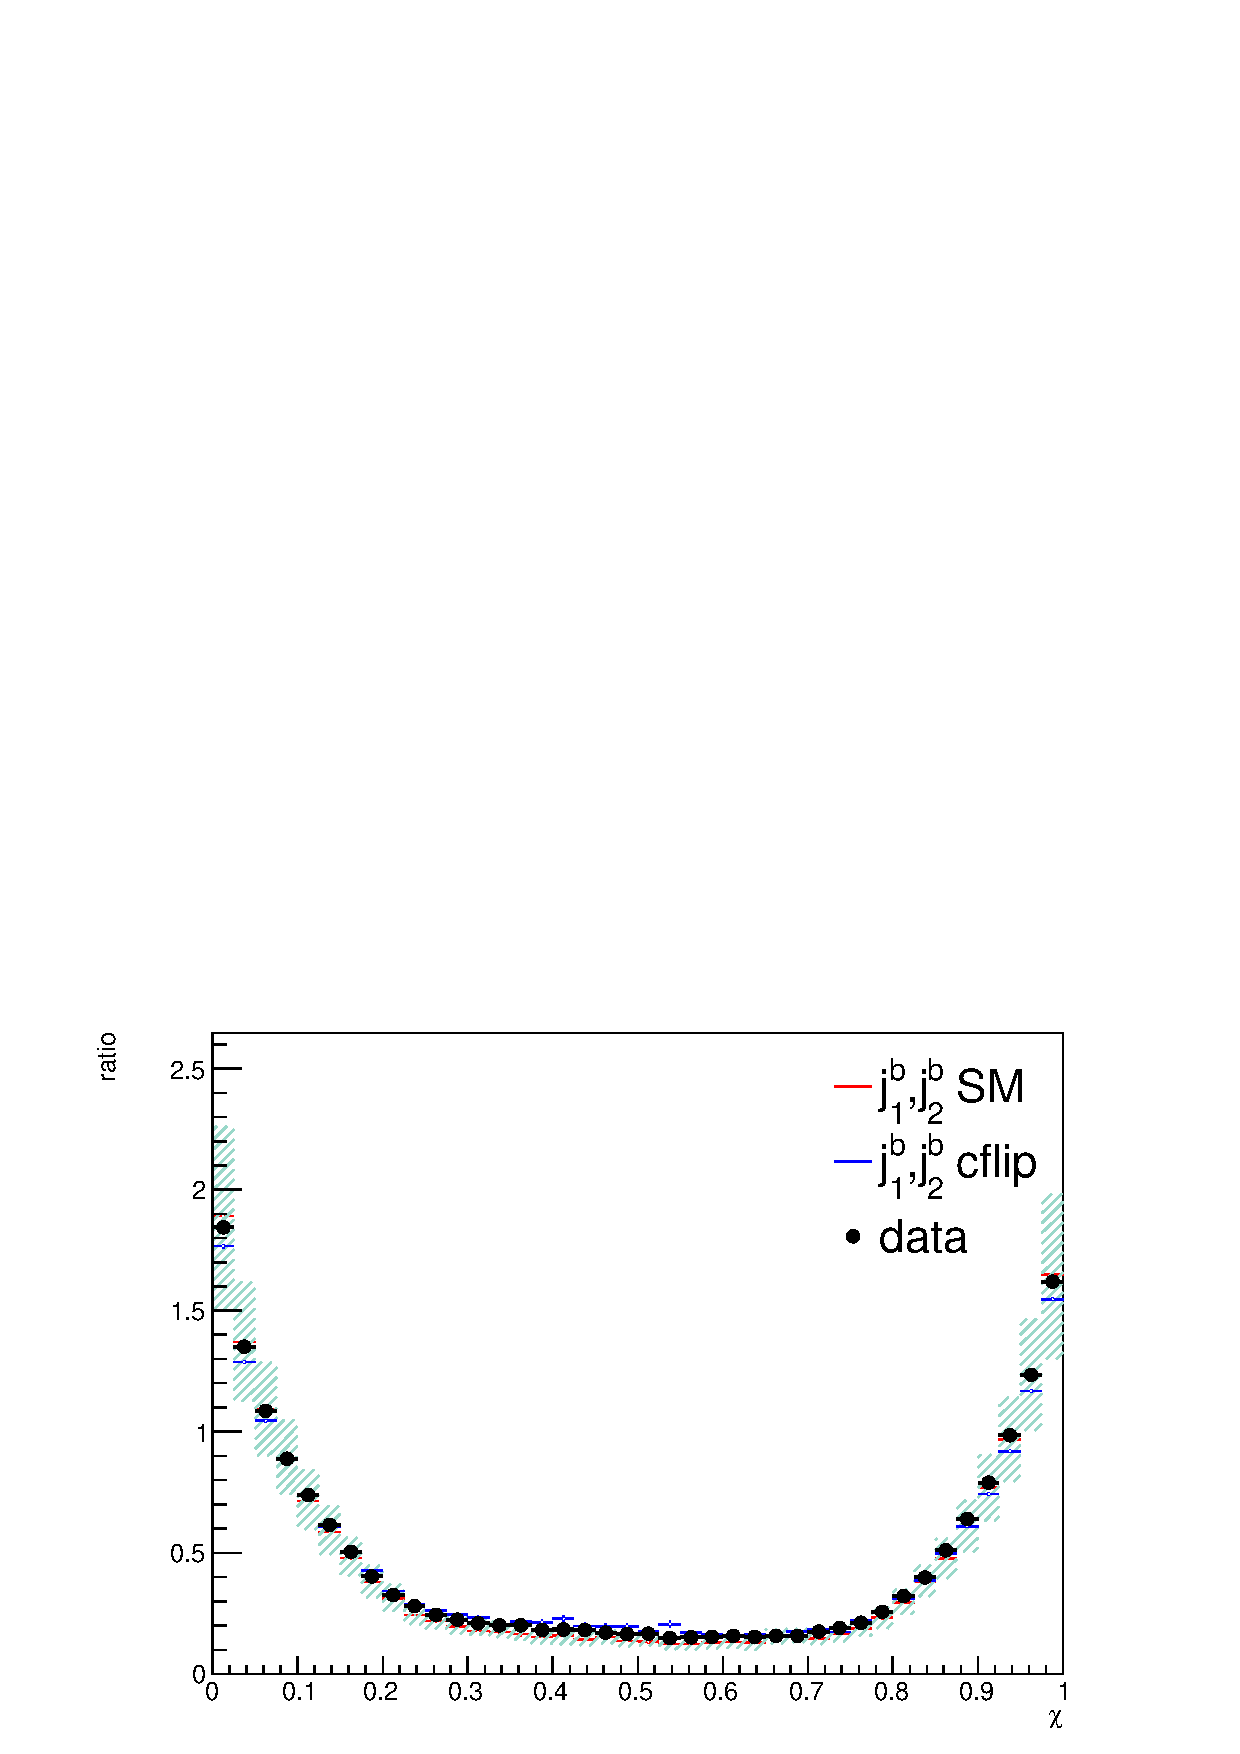
\includegraphics[width=\twidth\textwidth]{fig/ratiographs_merged_self/L_blb2l_N_allconst_reco.png}
    }%
    \subfloat[$j_{h}^{b}-j_{f}^{W}$]{
      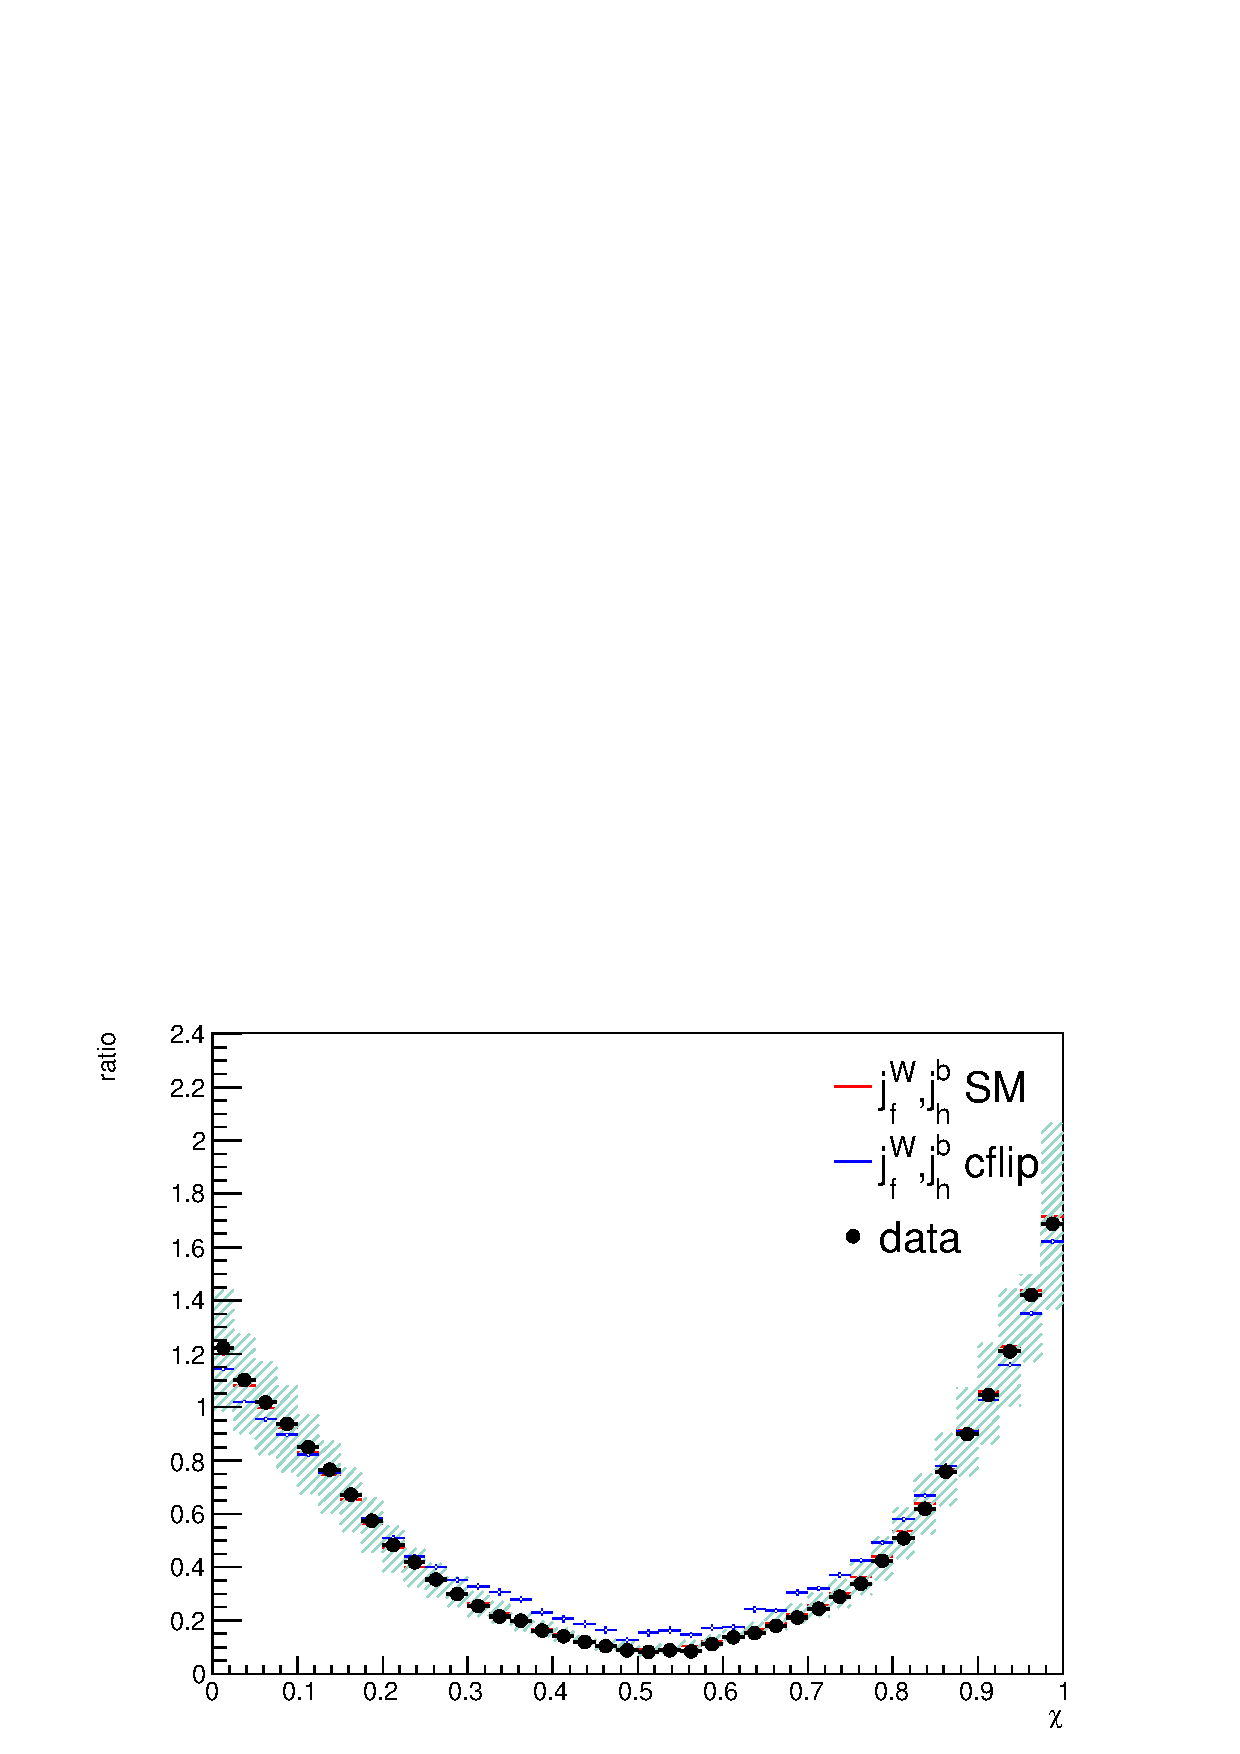
\includegraphics[width=\twidth\textwidth]{fig/ratiographs_merged_self/L_hbqf_N_allconst_reco.png}
    }%
    \subfloat[$j_{c}^{W}-j_{h}^{b}$]{
      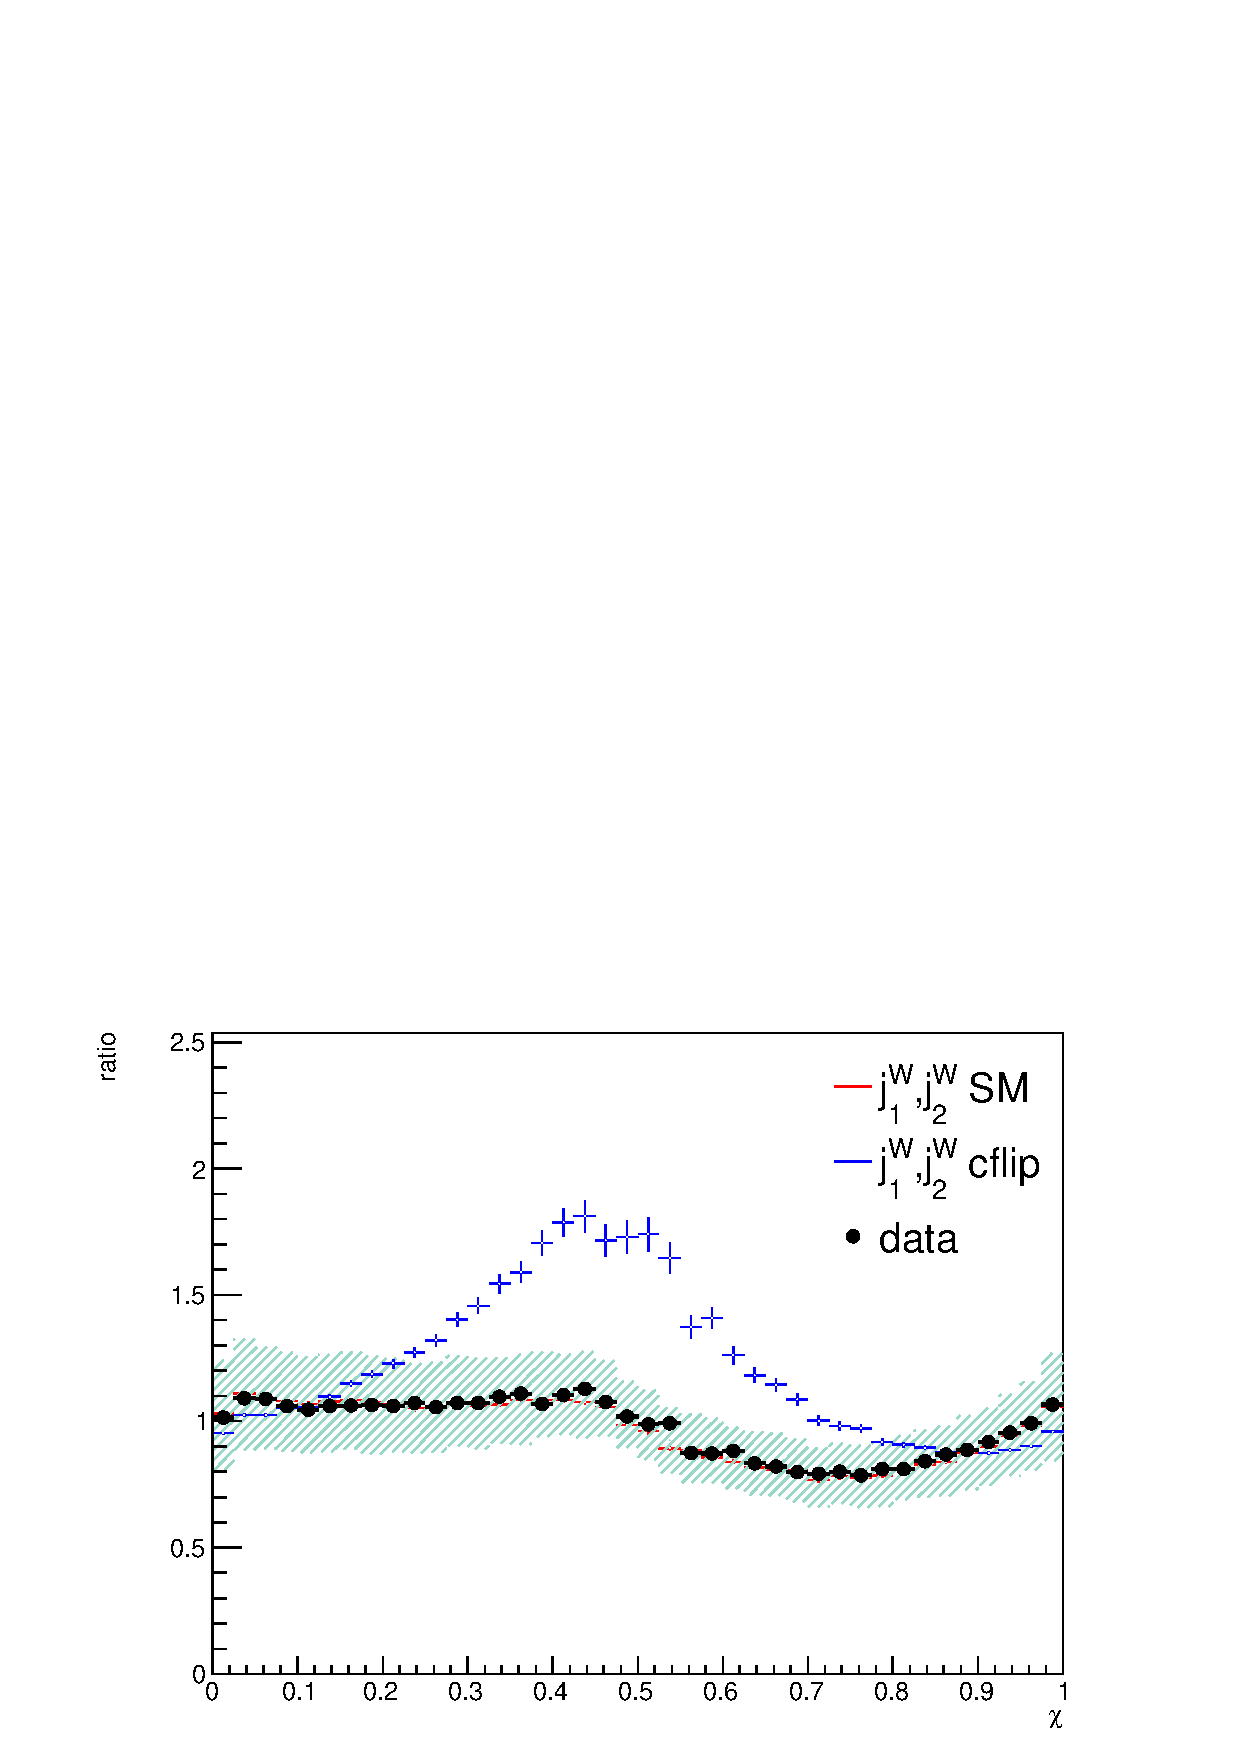
\includegraphics[width=\twidth\textwidth]{fig/ratiographs_merged_self/L_qcqf_N_allconst_reco.png}
    }%
  \end{figure}
\end{frame}

\begin{frame}{Krāsu okteta $W$ modeļa atiecība pret SM}
  \centering
  \includegraphics[width=0.8\textwidth]{fig/ratiographs_merged_SM/L_hbqc_N_allconst_reco.png}
\end{frame}

\begin{frame}
  \centering
  \begin{equation*}
    R=\frac{\int_{0.2}^{0.8}f^{\text{starp \PW reģions}}d\chi}{\int_{0.2}^{0.8}f^{\text{ārpus \PW reģions}}d\chi}
  \end{equation*}

  \scriptsize
  \input{nodalas_kopsavilkums/results/Rvalues_SMlv/R_L_reco_MC_N_SM.txt}
\end{frame}

\section{Hipotēžu pārbaude}

\begin{frame}{Modelis un testa statistika}
  2 hipotēžu modelis:
  \begin{equation*}
    n=\mu\left(\left(1-x\right)f_{t\overline{t}} + xf_{t\overline{t}_{\text{cflip}}}\right) + b
    \label{eq:two_hypo_model}
  \end{equation*}

  Neimana-Pīrsona testa statistika:

  \begin{equation*}
    q^{TEV}=-2\ln{\frac{L(H_{0})}{L(H_{\text{alt}})}}=-2\ln{\frac{L\left(\text{data}|p=0,\hat{\theta}_{0}\right)}{L\left(\text{data}|p=P,\hat{\theta}_{P}\right)}}
  \end{equation*}
  \end{frame}

\begin{frame}{PLR}
  \centering
  \includegraphics[width = 0.8\textwidth]{fig/likelihood}
\end{frame}

\begin{frame}{Testa statistikas sadalījums}
  \centering
  \includegraphics[width = 0.8\textwidth]{fig/hypo0p335.png}
  \begin{flushleft}
    p-vērtības:\\
    $H_{0}$: 0\\
    $H_{\text{alt}}$: 0,25
  \end{flushleft}
\end{frame}

\begin{frame}{Secinājumi}
  1. Krāsu saistību starp strūklām var novērot, izmantojot vilkmes leņķa vai ``LEP'' metodoloģiju\\
  2. Monte Karlo samērā neprecīzi modelē hadronizācijas procesu. Pythia gadījumā hromodinamiskie faktori tiek pārspīlēti. Hadronizācijas procesu labāk modelē Herwig ++, kā arī atsevišķi Pythia uzskaņojumi.\\
  3. Ar atlocīšanas metodi ieguvām patieso vilkmes leņķa sadalījumu, kas gan neietekmēja mūsu secinājumus par šīs metodes efektivitāti.\\
  4. Ar hipotēžu pārbaudes metodi noskaidrojām, ka atbilstību datiem vislabāk modelē Monte Karlo maisījums $\sim\frac{2}{3}$ $t\bar{t}$ un $\sim\frac{1}{3}$ $t\bar{t}$ cflip.
\end{frame}

\end{document}
